\documentclass{article}
\usepackage{graphicx} % Required for inserting images

\title{POO1}
\author{Juan E Osorno D.}
\date{March 2025}

\begin{document}

\maketitle

\section{Introduction}

We begin this section talking about the concept of template, in JAVA context we talk about class. Imagine a cube,
How many types of cubes exist? You will answer that a lot of them, and this is a good answer, because, if you are 
in minecraft game there are a lot of this cubes: dirt cube, stone cube, and a large etc... 

\begin{figure}[h!]
    \centering
    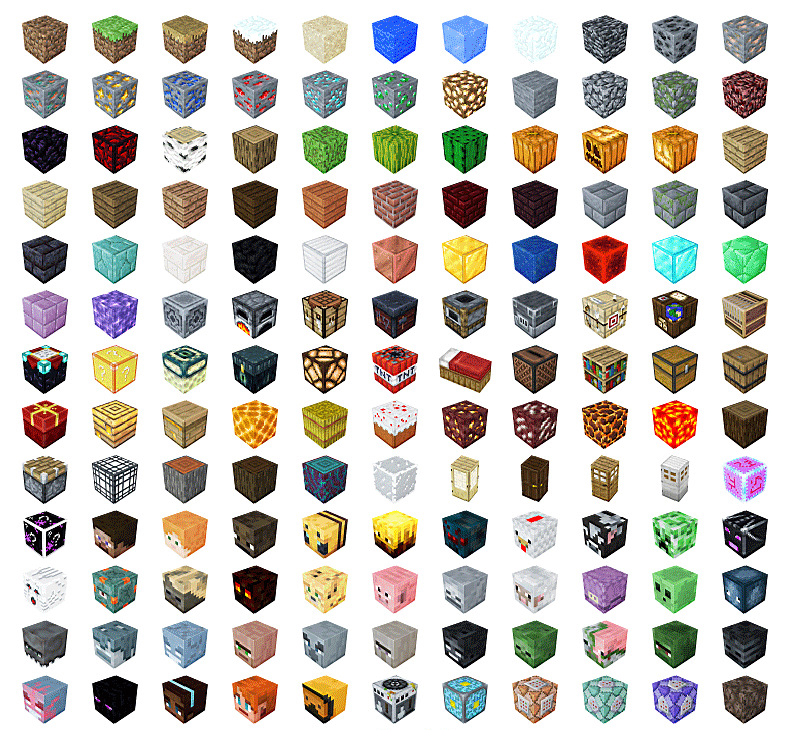
\includegraphics[width=0.5\textwidth]{Bloques.png}
    \caption{Minecraft Cubes}
    \label{fig:etiqueta}
\end{figure}

so in Minecraft context what is the property of all this cubes? If you see the figure 1, you can see that all of this cubes have different skins, so a attribute of a cube is the skin. Check out that we abstract the property of the cube and we arrive to its attribute. This is the next thing that we do after made a class: we abstract the concept of cube and define all things that a cube have. So A cube has a skin but this skin also has a name, for example the dirt cube has its name  and its skin. But what other property has a Cube? Think in its actions, for example its hardness: if you put this in a real context is not the same the hardness of a dirt cube vs stone cube. This is what we name a method. A method is a action that we can put to a class and open other thing that we can define about Object Orient Programming, this is the 
polymorphism, this is all actions that we can do over a class. 

Now we have the abstract, and the polymorphism, But what other 

\begin{figure}[h!]
    \centering
    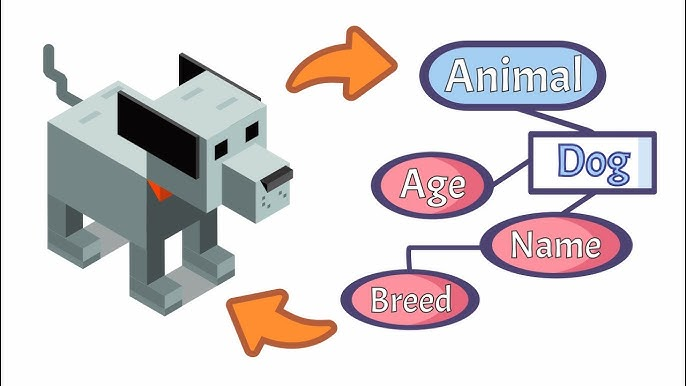
\includegraphics[width=0.5\textwidth]{hq720.jpg}
    \caption{Dog class}
    \label{fig:etiqueta}
\end{figure}

\end{document}